\begin{name}
	{\tenchude}
	{TOÁN 11}
	{LỚP TOÁN THẦY PHÁT}
	{Thời gian: 90 phút - Không kể thời gian phát đề}
\end{name}
\setcounter{ex}{0}\setcounter{bt}{0}
\TN
\Opensolutionfile{ans}[ans/ansDe2-TN1]
\begin{ex}%[1H8N1-1]
Trong không gian cho đường thẳng $\Delta$ và điểm $O$. Qua $O$ có bao nhiêu đường thẳng vuông góc với $\Delta$ cho trước?
\choice
{$1$}
{$2$}
{$3$}
{\True Vô số}
\loigiai{Qua $O$ có vô số đường thẳng vuông góc với $\Delta$ cho trước, tất cả các đường thẳng này cùng nằm trong mặt phẳng qua $O$ và vuông góc với đường thẳng $\Delta$ cho trước.}
\end{ex}

\begin{ex}%[BG - 10-11 New - 4in1, Phan Anh]%[1H8H4-2]
Cho hình chóp $S.ABC$ có đáy $ABC$ là tam giác vuông tại $B$,  $S A \perp (A B C)$. Khẳng định nào sau đây  đúng?
\choice
{$(SAC) \perp (SAB)$}
{$(SAC) \perp(SBC)$}
{\True $(SBC) \perp(SAB)$}
{$(SBC) \perp(ABC)$}
\loigiai{
\immini{
Vì $SA \perp (ABC)$ nên $SA\perp BC$. Mà $BC \perp AB$ suy ra $BC \perp (SAB)$. \\
Ta có $\heva{&BC \perp (SAB)\\& BC \subset (SBC)}$ $\Rightarrow (SBC) \perp (SAB)$.
}
{
\begin{tikzpicture}[scale=.8, font=\footnotesize, line join=round, line cap=round, >=stealth]
\path
(0,0)coordinate(A)
(1,-1)coordinate(B)
(3,0)coordinate(C)
($(A)+(0,2)$)coordinate(S);
\draw (S)--(A)--(B)--(S)--(C)--(B);
\draw [dashed](A)--(C) ;
\foreach \x/\g in{A/180,B/-90,C/0,S/90}
\fill[black](\x)circle(1.2pt) ($(\x)+(\g:3mm)$)node{$\x$};
\end{tikzpicture}
}
}
\end{ex}

\begin{ex}%[1H8H6-2]%[Dự án đề kiểm tra Toán 11 GHKI NH23-24-Võ Thị Thùy Trang]%[THPT MarieCurie- Tp HCM]
\immini{
Cho hình chóp $S.ABCD$ có đáy $ABCD$ là hình chữ nhật tâm $O$, $SA \perp(ABCD)$. Gọi $H$ là hình chiếu của $S$ lên $BD$. Góc phẳng nhị diện $[S, BD, A]$ là
\choice[2]
{$\widehat{SOA}$}
{$\widehat{SBA}$}
{\True $\widehat{SHA}$}
{$\widehat{SDA}$}
}
{\begin{tikzpicture}[>=stealth,line join=round,line cap=round,scale=1.0]
\draw[black,dashed] (0,0)coordinate(A)--(-130:1.5)coordinate(B) (3,0)coordinate(D)--(A)--($(A)+(90:3)$)coordinate(S);
\draw[black] (B)--($(D)-(A)+(B)$)coordinate(C)--(D)--(S)--(B) (S)--(C);
\coordinate (O) at ($(A)!0.5!(C)$);
\coordinate (H) at ($(B)!0.35!(D)$);
\draw[black,dashed] (A)--(C) (B)--(D) (S)--(H);
\path[black]
pic[angle radius=5,draw=blue,angle eccentricity=1.5] {right angle = S--H--B}
pic[angle radius=5,draw=blue,angle eccentricity=1.5] {right angle = D--A--S};
\foreach \diem/\vitrin in {S/above,A/left,B/below left,C/below right,D/right,O/above,H/below right} \fill (\diem)circle(.85pt)node[\vitrin]{$\diem$};
\end{tikzpicture}
}
\loigiai{
Ta có $SA \perp(ABCD)$ nên $BD \perp SA$.\\
Vì $H$ là hình chiếu của $S$ lên $BD$ nên $BD \perp SH$.\\
Do đó $BD \perp(SAH)$. Suy ra $BD \perp AH$.\\
Vậy góc phắng nhị diện $[S, BD, A]$ là $\widehat{SHA}$.
}
\end{ex}

\begin{ex}%[1H8H4-3]
Cho hình chóp $S.ABC$ có đáy là tam giác đều cạnh $a$. Hình chiếu vuông góc của $S$ lên $\left( ABC \right)$ là trung điểm của cạnh $BC$. Biết $\Delta SBC$ đều, góc giữa hai mặt phẳng $\left( SAB \right)$ và $\left( ABC \right)$ bằng
\choice
{\True $60^\circ $}
{$45^\circ $}
{$90^\circ $}
{$30^\circ $}
\loigiai{
\immini{
Gọi $M$ là trung điểm của $BC$. Khi đó $SM\perp \left( ABC \right)$.\\
Gọi $H$ là trung điểm của $AB\Rightarrow HM\perp AB$.\\
Ta có $\heva{
&\left( SAB \right)\cap \left( ABC \right)=AB \\
&AB\perp MH,MH\subset \left( ABC \right) \\
&AB\perp SH,SH\subset \left( SAB \right) \\
}$ \\$\Rightarrow \bigl( \left( SAB \right),\left( ABC \right) \bigr)=\widehat{SHM}$\\
Tam giác $SAB$ đều nên $SM=\dfrac{a\sqrt 3} 2$.\\
Tam giác $ABC$ đều nên $HM=\dfrac{a}{2}$.\\
}
{
\begin{tikzpicture}[line join=round,line cap=round,line width=.6pt,font=\footnotesize,scale=1]
\coordinate[label=left:$A$] (A) at (0,0);
\coordinate[label=below left:$B$] (B) at (1,-1);
\coordinate[label=right:$C$] (C) at (4,0);
\coordinate[label=below right:$M$] (M) at ($(B)!.5!(C)$);
\coordinate[label=below:$H$] (H) at ($(A)!1/2!(B)$);
\coordinate[label=above :$S$] (S) at ($(M)+(90:3)$);
\draw (A)--(B)--(C)--(S)--cycle (S)--(B) (H)--(S)--(M);
\draw[dashed] (M)--(A)--(C) (M)--(H);
\fill (A)circle(2pt) (B)circle(2pt) (C)circle(2pt) (S)circle(2pt) (H)circle(2pt) (M)circle(2pt);
\end{tikzpicture}
}

Tam giác $SHM$ vuông tại $M$ có $\tan \widehat{SHM}=\dfrac{SM}{HM}=\dfrac{\dfrac{a\sqrt 3} 2}{\dfrac{a}{2}}=\sqrt 3$.\\
$\Rightarrow \widehat{SHM}=60^\circ $ nên góc giữa hai mặt phẳng $\left( SAB \right)$ và $\left( ABC \right)$ bằng $60^\circ $.
}
\end{ex}

\begin{ex}%[1H8N6-2]%[Dự án đề kiểm tra Toán 11 GHKI NH23-24- Tổng Nguyễn]%[THPT Phạm Phú Thứ - Đà Nẵng]
Số đo của góc nhị diện có thể nhận giá trị từ
\choice
{\True  $0^\circ$ đến $180^\circ$ }
{  $0^\circ$ đến $90^\circ$ }
{  $90^\circ$ đến $180^\circ$ }
{  $180^\circ$ đến $360^\circ$ }
\loigiai{
Số đo của góc nhị diện có thể nhận giá trị từ $0^\circ$ đến $180^\circ$. }
\end{ex}

\begin{ex}%[1H8N4-1]
Mệnh đề nào sau đây là đúng?
\choice
{Hai mặt phẳng vuông góc với nhau thì mọi đường thẳng nằm trong mặt phẳng này sẽ vuông góc với mặt phẳng kia}
{Hai mặt phẳng phân biệt cùng vuông góc với một mặt phẳng thì vuông góc với nhau}
{Hai mặt phẳng phân biệt cùng vuông góc với một mặt phẳng thì song song với nhau}
{\True Hai mặt phẳng vuông góc với nhau thì mọi đường thẳng nằm trong mặt phẳng này và vuông góc với giao tuyến của hai mặt phẳng sẽ vuông góc với mặt phẳng kia}
\loigiai{
\begin{itemize}
\item Mệnh đề \lq\lq  Hai mặt phẳng vuông góc với nhau thì mọi đường thẳng nằm trong mặt phẳng này sẽ vuông góc với mặt phẳng kia\rq\rq\, sai vì có thể xảy ra trường hợp hai mặt phẳng vuông góc với nhau nhưng đường thẳng thuộc mặt phẳng này song song với mặt phẳng kia.
\item Mệnh đề \lq\lq  Hai mặt phẳng phân biệt cùng vuông góc với một mặt phẳng thì vuông góc với nhau\rq\rq\, sai vì xảy ra trường hợp hai mặt phẳng song song.
\item Mệnh đề \lq\lq  Hai mặt phẳng phân biệt cùng vuông góc với một mặt phẳng thì song song với nhau\rq\rq\, sai vì xảy ra trường hợp hai mặt phẳng vuông góc.
\end{itemize}
}
\end{ex}

\begin{ex}%[1H8H2-2]
Cho hình chóp $S.ABCD$ có đáy $ABCD$ là hình chữ nhật, $SA\perp\left(ABCD\right)$. Gọi $H,K$ lần lượt là hình chiếu của $A$ lên $SC$, $SD$. Khẳng định nào sau đây đúng?
\choice
{$BC\perp\left(SAC\right)$}
{$BD\perp\left(SAC\right)$}
{$AH\perp\left(SCD\right)$}
{\True $AK\perp\left(SCD\right)$}
\loigiai
{
\immini
{
Ta có $\heva{&SA\perp CD \\&AD\perp CD}\Rightarrow CD\perp \left(SAD\right)\Rightarrow CD\perp AK$.\\
Lại có $SD\perp AK$.\\
Suy ra $AK\perp \left(SCD\right)$.
}
{
\begin{tikzpicture}[line join=round, line cap=round,thick]
\coordinate (A) at (0,0);
\coordinate (B) at (-2,-1);
\coordinate (D) at (3,0);
\coordinate (C) at ($(B)+(D)-(A)$);
\coordinate (S) at ($(A)+(0,3)$);
\coordinate (H) at ($(S)!0.4!(C)$);
\coordinate (K) at ($(S)!0.4!(D)$);
\draw(S)--(B) (S)--(C) (S)--(D) (B)--(C)--(D);
\draw[dashed,thin](S)--(A) (A)--(B) (A)--(D) (A)--(H) (A)--(K);
\pic[draw,thin,angle radius=2mm] {right angle = S--A--D} pic[draw,thin,angle radius=2mm] {right angle = S--A--B}
pic[draw,thin,angle radius=2mm] {right angle = S--K--A}
pic[draw,thin,angle radius=2mm] {right angle = S--H--A};
\foreach \i/\g in {S/90,A/-90,B/-90,C/-90,D/0,H/45,K/45}{\draw[fill=white](\i) circle (1pt) ($(\i)+(\g:3mm)$) node[scale=1]{$\i$};}
\end{tikzpicture}
}
}
\end{ex}

\begin{ex}%[1D6N3-1]%[Dự án đề kiểm tra Toán 11 CKII NH23-24- Hoàng Vũ]%[THPT TRẦN ĐẠI NGHĨA - HCM]
Hàm số nào sau đây là hàm số mũ?
\choice
{$y=\sqrt[3]{x}$}
{$y=x^3$}
{$y=(\sin x)^3$}
{\True$y=3^x$}
\loigiai{
Hàm số mũ có dạng $y=a^x$ với $a>0$, do đó đáp án hàm số $y=3^x$ là đúng.}
\end{ex}

\begin{ex}%[1H8N6-1]%[Dự án đề kiểm tra Toán 11 HK II NH23-24 - Nguyễn Thành Sơn]%[THPT Nguyễn Thái Bình - Tp.HCM]
Cho hình chóp $S.ABCD$ có đáy $ABCD$ là hình vuông, $SA \perp(ABCD)$. Khi đó góc giữa đường thẳng $SD$ và mặt phẳng $(ABCD)$ là góc giữa hai đường thẳng
\choice
{\True $S D$ và $A D$}
{$S D$ và $S A$}
{$S D$ và $B D$}
{$S D$ và $C D$}
\loigiai{
\immini{
Ta có $SA\perp (ABCD)$ $\Rightarrow AD$ là hình chiếu vuông góc của $SD$ lên $(ABCD)$.\\
Suy ra, góc giữa đường thẳng $SD$ và mặt phẳng $(ABCD)$ là góc giữa hai đường thẳng  $SD$ và $AD$.
}{\begin{tikzpicture}[scale=.75, font=\footnotesize, line join=round, line cap=round, >=stealth]
\def\a{2.75}
\def\b{2}
\def\h{2.5}
\def\g{120}
\path (0,0) coordinate (A) (0:\a) coordinate (D) --++(-\g:\b) coordinate (C) --++(-180:\a)coordinate (B);
\coordinate (O) at ($(A)!1/2!(C)$);
\coordinate (S) at ($(A)+(0,\h)$);
\coordinate (H) at ($(S)!(A)!(D)$);
\draw (B)--(C)--(D)--(S)--(B) (S)--(C) ;
\draw[dashed] (S)--(A)--(D)--(B)--(A)--(C) ;
\foreach \x/\g in {A/45,B/-90,C/-90,D/0,S/90}  \fill (\x) circle (1pt)+(\g:.25)node {$\x$};
\end{tikzpicture}}


}
\end{ex}

\begin{ex}%[1D6N2-2]
Với $ a$ là số thực khác $0$ tùy ý, $\log_2a^2$ bằng
\choice
{$a$}
{$2\log_2a$}
{\True $2\log_2|a|$}
{$\dfrac{1}{2}\log_2a$}
\loigiai{
Ta có $\log_2a^2=2\log_2|a|$ .}
\end{ex}

\begin{ex}%[1H8N2-1]
Khẳng định nào sau đây \textbf{sai}?
\choice
{Nếu đường thẳng $d$ vuông góc với mặt phẳng $(\alpha)$ thì $d$ vuông góc với hai đường thẳng trong mặt phẳng $(\alpha)$}
{\True Nếu đường thẳng $d$ vuông góc với hai đường thẳng nằm trong mặt phẳng $(\alpha)$ thì $d$ vuông góc với mặt phẳng $(\alpha)$}
{Nếu đường thẳng $d$ vuông góc với hai đường thẳng cắt nhau nằm trong mặt phẳng $(\alpha)$ thì $d$ vuông góc với bất kỳ đường thẳng nào nằm trong mặt phẳng $(\alpha)$}
{Nếu $d\perp(\alpha)$ và đường thẳng $a\parallel (\alpha)$ thì $d\perp a$}
\loigiai{
Khẳng định “Nếu đường thẳng $d$ vuông góc với hai đường thẳng nằm trong mặt phẳng $(\alpha)$ thì $d$ vuông góc với mặt phẳng $(\alpha)$” sai vì: đường thẳng $d$ vuông góc với hai đường thẳng nằm trong mặt phẳng $(\alpha)$ mà hai đường thẳng đó song song thì $d$ không vuông góc với mặt phẳng $(\alpha)$.
}
\end{ex}

\begin{ex}%[1D6N1-2]%[Dự án đề kiểm tra Toán 11 HK2 NH23-24- Nguyễn Hữu Duy]%[THPT Chuyên Hùng vương - Phú Thọ]
Cho $a$ là số thực dương. Rút gọn biểu thức $A = \dfrac{\sqrt{a}}{\sqrt[3]{a}}$, ta được kết quả là
\choice
{\True $a^{\frac{1}{6}}$}
{$a$}
{$a^{-1}$}
{$a^{\frac{5}{6}}$}
\loigiai{
Ta có $A = \dfrac{\sqrt{a}}{\sqrt[3]{a}} = \dfrac{a^{\frac{1}{2}}}{a^{\frac{1}{3}}} = a^{\frac{1}{2} = \frac{1}{3}} = a^{\frac{1}{6}}$.
}
\end{ex}
\Closesolutionfile{ans}

\TNTF
\Opensolutionfile{ans}[ans/ansDe2-TN2]
\begin{ex}%[1D6H2-3]
Cho các biểu thức sau $P=\dfrac{\log _a\left(a^3 b^2\right)-\log _b\left(\dfrac{b^3}{a^2}\right)}{\log _a^2 b+1}$và $Q=\log_ab^3+\log_{a^2}b^6$ với $a, b$ là các số dương và $a$ khác $1$. Vậy
\choiceTF
{\True $Q=6\log_ab$}
{$P=6\log_ba$}
{$Q=3P$}
{\True $Q\cdot P=12$}
\loigiai{
Ta có $Q=3\log_ab+6\cdot \dfrac{1}{2}\log_ab=6\log_ab$.\\
Ta có \begin{eqnarray*}
&P&=\dfrac{\log _a a^3+\log _a b^2-\left(\log _b b^3-\log _b a^2\right)}{\log _a^2 b+1}\\
&&=\dfrac{3+2 \log _a b-3+2 \log _b a}{\log _a^2 b+1}\\
&&=\dfrac{2\left(\log _a b+\dfrac{1}{\log _a b}\right)}{\log _a^2 b+1}\\
&&=\dfrac{2\left(\dfrac{\log _a^2 b+1}{\log _a b}\right)}{\log _a^2 b+1}\\
&&=\dfrac{2}{\log _a b}=2 \log _b a.
\end{eqnarray*}
Do đó
\begin{itemchoice}
\itemch Đúng. Vì $Q=6\log_ab$.
\itemch Sai. Vì $P=2\log_ba\neq 6\log_ba$.
\itemch Sai. Vì $Q=6\log_ab\neq 3\cdot 2\log_ba=3P$.
\itemch Đúng. Vì $Q\cdot P=6\log_ab\cdot 2\log_ba=12$.
\end{itemchoice}
}
\end{ex}

\begin{ex}%[1H8H6-1]
Cho hình chóp $S.ABC$ có $SA\perp (ABC)$, $AB\perp BC$, $SA=AB=a$, $AC=a\sqrt{3}$ (như hình vẽ).
\immini{
\choiceTF [t]
{\True $BC\perp (SAB)$}
{Góc giữa đường thẳng $SC$ và mặt phẳng $(SAB)$ bằng $\widehat{CSA}$}
{\True $\tan\widehat{CSB}=1$}
{Góc giữa đường thẳng $SC$ và mặt phẳng $(SAB)$ bằng $60^\circ$}
}
{\begin{tikzpicture}[line join=round,line cap=round,>=stealth,scale=0.8,font=\footnotesize]
\tikzset{every node/.style={outer sep=-0.5mm}}
\foreach \x/\y/\n in {0/0/A,5/0/C,2/-2/B} \coordinate (\n) at (\x,\y);
\coordinate (S) at ($(A)+(0,3.5)$);
\draw (S)--(A)node[midway,left]{$a$}--(B)node[midway,below left]{$a$}--(C)--(S)--(B);
\draw[dashed] (A)--(C)node[midway,above]{$a\sqrt{3}$};
\draw pic[thin,draw,angle radius=2mm] {right angle= C--B--A};
\foreach \t/\g in {A/180,B/-90,C/0,S/90}{
\draw[fill=black] (\t) circle (1pt) node[shift={(\g:8pt)}]{$ \t $};
}
\end{tikzpicture}}
\loigiai{
\begin{itemchoice}
\itemch Đúng.\\
Ta có $\heva{&SA\perp BC\text{ do }SA\perp(ABC)\\&AB\perp BC}\Rightarrow BC\perp(SAB)$.
\itemch Sai.\\
Ta có $BC\perp(SAB)\Rightarrow SB$ là hình chiếu vuông góc của $SC$ trên $(SAB)$.\\
Do đó $(SC,(SAB))=(SC,SB)=\widehat{CSB}$.
\itemch Đúng.\\
Ta có $\triangle SBC$ vuông tại $B$. Khi đó
\[\tan \widehat{CSB}=\dfrac{BC}{SB}=\dfrac{\sqrt{AC^2-AB^2}}{SA^2+AB^2}=\dfrac{\sqrt{3a^2-a^2}}{\sqrt{a^2+a^2}}=\dfrac{a\sqrt{2}}{a\sqrt{2}}=1.\]
\itemch Sai.\\
Ta có góc giữa đường thẳng $SC$ và mặt phẳng $(SAB)$ bằng $\widehat{CSB}$.\\
Mà $\tan \widehat{CSB} =1 \Rightarrow \widehat{CSB}=45^\circ$.
\end{itemchoice}
}
\end{ex}
\Closesolutionfile{ans}

\TNSA
\Opensolutionfile{ans}[ans/ansDe2-TN3]
\begin{ex}%[1D6N3-1]%[tex hóa đề ck2 - form 2025 - đợt 2 - Hồ Văn Trung]
	Đường cong trong hình bên là của đồ thị hàm số $y=a^x$ (với $a>0$). Giá trị biểu thức $a^2$ bằng
	\begin{center}
	\begin{tikzpicture}[line join=round, line cap = round, >=stealth, scale=0.7,font=\footnotesize,transform shape]
	\draw[->] (-3,0)--(3,0) node[below]{$x$};
	\draw[->] (0,-1)--(0,5) node[right]{$y$};
	\draw (0,0)node[below right]{$O$};
	\draw[samples=100,smooth,domain=-3:3] plot(\x,{(0.6)^(\x)});
	\draw[dashed] (1,0)node[below]{$1$}|-(0,0.6)node[right]{$0,6$};
	\end{tikzpicture}
	\end{center}
	\shortans{$0{,}36$}
	\loigiai{
		Ta có $a^2=0{,}6^2=0{,}36$.
	}
	\end{ex}

	\begin{ex}%[1D6H4-5]
		Tập nghiệm $S$ của bất phương trình $\log_{\tfrac{1}{5}}(x+1) < \log_{\tfrac{1}{5}}(2x-1)$ là $(a;b)$. Giá trị của $a+b$ bằng
		\shortans{$2,5$}
		\loigiai{
		Điều kiện $x > \dfrac{1}{2}$.\\
		Ta có $\log_{\tfrac{1}{5}}(x+1) < \log_{\tfrac{1}{5}}(2x-1) \Leftrightarrow x+1 > 2x-1 \Leftrightarrow x < 2$.\\
		Kết hợp điều kiện bất phương trình có tập nghiệm $S=\left(\dfrac{1}{2}; 2\right)$.
		}
		\end{ex}

\begin{ex}%[1H8V6-7]
	Kim tự tháp Memphis tại bang Tennessee (Mỹ) có dạng hình chóp tứ giác đều với chiều cao $98$ m và cạnh đáy $180$ m. Tính số đo góc nhị diện tạo bởi mặt bên và mặt đáy của kim tự tháp đó. (đơn vị đo góc là độ, làm tròn đến hàng phần chục)
	\shortans{$47{,}4$}
	\loigiai{

	\begin{center}
		\begin{tikzpicture}
			\path
			(0,0) coordinate[label=left: A] (A)
			(-1,-1) coordinate[label=left: B] (B)
			(3,0) coordinate[label=right: D] (D)
			(2,-1) coordinate[label=right: C] (C)
			(1,3) coordinate[label=above: S] (S)
			($(A)!0.5!(C)$) coordinate[label=below: O] (O)
			;
			\draw (D)--(C)--(B);
			\draw[dashed] (B)--(A)--(D);
			\draw[dashed] (A)--(C) (D)--(B);
			\draw[dashed] (S)--(A);
			\draw (B)--(S)--(C)  (D)--(S);


		\end{tikzpicture}
	\end{center}
	Xét hình chóp tứ giác đều $S.ABCD$ có chiều cao $98$ m và cạnh đáy $180$ m.\\
	Gọi $O$ là tâm hình vuông $ABCD$ thì $SO\perp (ABCD)\Rightarrow SO\perp AB$.\hfill $(1)$\\
	Gọi $M$ là trung điểm $AB$ thì $OM$ là đường trung bình của tam giác $ABC$, \\
	Suy ra $OM=\dfrac{BC}{2}=90$ (m) và $OM\perp AB.$\hfill $(2)$\\
	Từ $(1)$ và $(2)$ suy ra $\widehat{SMO}$ là góc phẳng nhị diện $[S,AB,O]$ \\
	với \[\tan \widehat{SMO}=\dfrac{SO}{OM}=\dfrac{98}{90}=\dfrac{49}{45} \Rightarrow \widehat{SMO}\approx 47{,}44^{\circ}\]
	Vậy góc nhị diện tạo bởi mặt bên và mặt đáy của kim tự tháp xấp xỉ $47{,}44^{\circ}$.
	}
\end{ex}

\begin{ex}%[1D6V1-2]
Dân số sau $n$ năm được tính theo công thức $P_n=P_0 \cdot e^{nr}$, trong đó $P_0$ là dân số của năm lấy làm mốc tính, $r$ là tỉ lệ tăng dân số hàng năm. Biết rằng năm $2020$, dân số thế giới là $7{,}795$ tỉ người (nguồn: \textit{https://danso.org/dan-so-the-gioi-theo-nam}). Giả sử tỉ lệ tăng dân số hàng năm của thế giới là $1{,}05\%$. Hỏi dân số thế giới vào năm $2035$ là bao nhiêu tỉ người? (kết quả làm tròn đến hàng phần trăm)
\shortans{$9,12$}
\loigiai{
Vào năm $2020$ (sau $n_1$ năm tính từ năm lấy làm mốc), dân số thế giới là $7{,}795$ tỉ người nên $P_{n_1}=P_0 \cdot e^{n_1 \cdot r}=7{,}795$.\\
Vào năm $2035$ (sau $n_2$ năm tính từ năm lấy làm mốc), dân số thế giới là là $P_{n_2}=P_{0}\cdot e^{n_2 \cdot r}$.\\
Ta có
\begin{align*}
&\dfrac{P_{n_2}}{P_{n_1}}=\dfrac{P_0 \cdot e^{n_2 \cdot r}}{P_0 \cdot e^{n_1 \cdot r}}=e^{(n_2-n_1) r}=e^{{(2035-2020) \cdot 1{,}05\%}}=e^{15  \cdot 1{,}05\%} \\
&\Rightarrow P_{n_2}= e^{15  \cdot 1{,}05\%} \cdot P_{n_1}= e^{15  \cdot 1{,}05\%} \cdot 7{,}795 \approx 9{,}12.
\end{align*}
Vậy dân số thế giới vào năm $2035$ đạt khoảng $9{,}12$ tỉ người.}
\end{ex}


\Closesolutionfile{ans}

\TL
\begin{ex}%[1D6H4-4]%[Dự án đề kiểm tra Toán 11 GHKI NH23-24-Nguyễn Tài Tuệ]%[THPT PhamVanSang - Tp HCM]
Giải phương trình $2 \log _2(x-1)+\log _{\tfrac{1}{2}}(5-x)=1$.
\loigiai{
Điều kiện xác định $\heva{&x-1>0\\& 5-x>0}\Leftrightarrow 1<x<5 $.\\
Với điều kiện đó phương trình tương đương với
\begin{eqnarray*}
&&\log _2(x-1)^2-\log_{2}(5-x)=1\\
&\Leftrightarrow&\log_2\dfrac{(x-1)^2}{5-x}=1\\
&\Leftrightarrow&\dfrac{(x-1)^2}{5-x}=2\\
&\Leftrightarrow&x^2-2x+1=10-2x\\
&\Leftrightarrow&x^2=9\\
&\Leftrightarrow&x=\pm 3.
\end{eqnarray*}
Đối chiếu với điều kiện suy ra nghiệm của phương trình $x=3$.
}
\end{ex}

\begin{ex}%[1D6H4-6]
	Số lượng loại vi khuẩn $A$ trong một phòng thí nghiệm được tính theo công thức $s(t)=s(0)\cdot 2^t$, trong đó $s(0)$ là số lượng vi khuẩn $A$ lúc ban đầu, $s(t)$ là số lượng vi khuẩn $A$ có sau $t$ phút. Biết sau $3$ phút thì số vi khuẩn $A$ là $625$ nghìn con. Hỏi sau bao lâu kể từ lúc ban đầu, số lượng loại vi khuẩn $A$ là $20$ triệu con.
	% \shortans[0]{8}
	\loigiai{
	Theo giả thiết ta có: $s(3)=625\,000\Leftrightarrow s(0)\cdot 2^3=625\,000\Leftrightarrow s(0)=78\,125$.\\
	Số lượng loại vi khuẩn $A$ là 20 triệu con khi\\
	$s(t)=20\,000\,000\Leftrightarrow s(0)\cdot 2^t=20\,000\,000
	\Leftrightarrow {2^t}=\dfrac{20\,000\,000}{s(0)}=\dfrac{20\,000\,000}{78\,125}=256
	\Leftrightarrow t=8$.\\
	Vậy sau $8$ phút thì số lượng vi khuẩn $A$ là $20$ triệu con.
	}
	\end{ex}

	\begin{ex}%[1H8C2-4]
		\immini{Cho tứ diện $ABCD$ có $AB=x$, $(x>0)$, các cạnh còn lại bằng nhau và bằng $4$. Mặt phẳng $(P)$ chứa cạnh $AB$ và vuông góc với cạnh $CD$ tại $I$. Khi diện tích tam giác $IAB$ lớn nhất thì $x=\sqrt{a}$. Tìm $a$.}
		{
		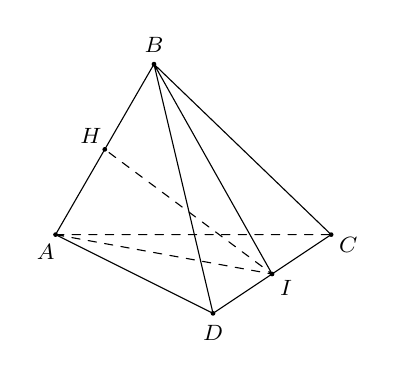
\begin{tikzpicture}[scale=1,>=stealth, font=\footnotesize, line join=round, line cap=round,declare function={h=2.5;}]
		\path
		(0,0) coordinate (A)
		(2,-1) coordinate (D)
		(3.5,0) coordinate (C)
		(A)+(60:h) coordinate (B)
		(barycentric cs:C=1,D=1)coordinate(I)
		(barycentric cs:A=1,B=1)coordinate(H)
		;
		\draw[dashed] (A)--(C) (A)--(I)--(H);
		\draw (I)--(B)--(D)--(A)--(B)--(C)--(D);
		\foreach \p/\g in{A/-120,B/90,C/-30,D/-90,I/-45,H/135}
		\fill[black](\p)circle(.03)node[shift={(\g:.25)},scale=1]{$\p$};
		\end{tikzpicture}
		}
		% \shortans{$24$}
		\loigiai{
		Ta có $(P)\perp CD$ tại $I$ nên $AI\perp DC$, $BI\perp DC$. Từ giả thiết $AD=AC=BC=BD=CD=4$ ta có các tam giác $\triangle ACD$, $\triangle BCD$ là các tam giác đều cạnh $4$. Suy ra $IA=IB=4\dfrac{\sqrt{3}}{2}=2\sqrt{3}$. Gọi $H$ là trung điểm của $AB$, ta có $IH\perp AB$ và\\
		$IH=\sqrt{IA^2-\dfrac{x^2}{4}}=\sqrt{12-\dfrac{x^2}{4}}$.\\ $S_{\triangle IAB}=\dfrac{1}{2}IH. AB=\dfrac{1}{2}x\sqrt{12-\dfrac{x^2}{4}}=\sqrt{\dfrac{x^2}{4}\left(12-\dfrac{x^2}{4}\right)}\le 6$.\\
		Vậy $\max S_{\triangle IAB}=6$, dấu \lq\lq =\rq\rq~xảy ra khi và chỉ khi $x=2\sqrt{6}=\sqrt{24}$. Vậy $a=24$.
		}
		\end{ex}

% \Closesolutionfile{ansbook}
% \HetDe
% \label{De2}
% %
% \cleardoublepage
% \setcounter{page}{1}
% \rfoot{Trang \thepage/\pageref{DA2} - Đáp án trắc nghiệm Mã đề 2}
% \begin{center}
% 	\bfseries ĐÁP ÁN TRẮC NGHIỆM MÃ ĐỀ 2
% \end{center}

% \inputansbox{10}{ans/ansDe2-TN1}
% \inputansbox[3]{2}{ans/ansDe2-TN2}
% \inputansbox{3}{ans/ansDe2-TN3}
% \label{DA2}
%
